\chapter{Background}  %remove chapter or use "part"
The aim of this work is to create a model that predicts if an article comment or a forum post can be classified as "persuasive" or "non-persuasive". We'll first give general definitions about persuasion and argumentation, and how the corpus was annotated. Then, the tool that was used to perform the classfication, DKPro Text Classification Framework, will be introduced and its functionnalities will be explained. Finally we'll discuss about the algorithm used and the metrics to evaluate our model.
\section{Argumentation}  %% To be changed while writting it
\subsection{General Definitions}
\subsection{Persuasion}
\subsection{Persuasion 2.0} %euh ?

\section{NLP and the DKPro Framework}
\subsection{Natural Language Processing}
%% Find something to say with some references
\subsection{UIMA}
DKPro stands for \emph{Darmstadt Knowledge Processing}
\cite{GurevychEtal2007dkpro0} and it's a software suite for NLP based on the Apache UIMA Framework. UIMA are software systems that analyse large volumes of unstructured information in order to discover knowledge that is relevant to an end user. An example UIMA application might ingest plain text and identify entities, such as persons, places, organizations; or relations, such as works-for or located-at:

\
\begin{figure}[ht]
    \centering
    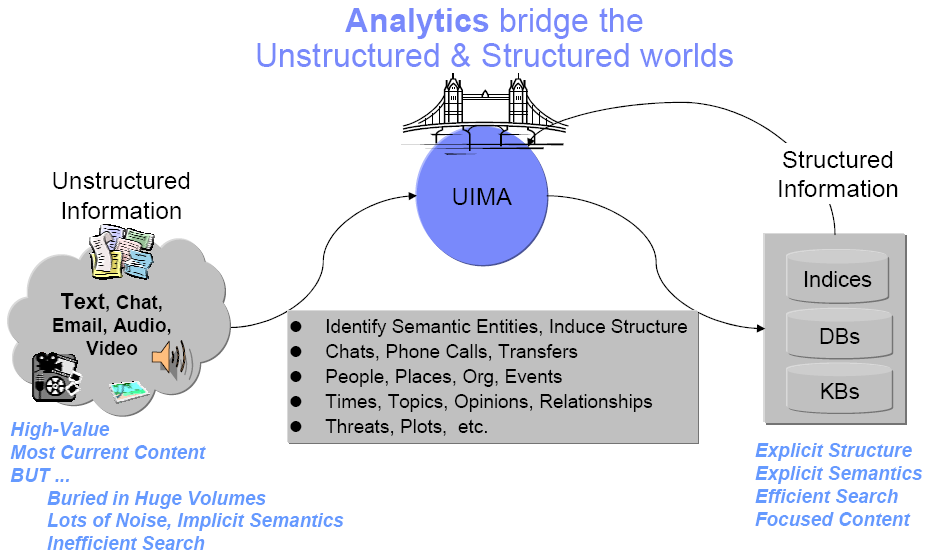
\includegraphics[width=1\textwidth]{fig/uima.png}
    \caption[Short caption]{UIMA: Order unstructured data, from UIMA website \cite{uima:Online}}
    \label{fig:uima}
\end{figure}
\

The real power of UIMA is its Analysis Engines (AE) which basically analyse a document and record descriptive attributes. Those descriptive attributes will form the document's metadata that will be used for further analysis (such as Text Classification in our case).

GIVE EXAMPLES OF AE HERE AND DKPRO PROC PIPILINE AND CAS ?

Thus, the DKPRo software use UIMA's AE in order to collect structured information about textual data. 
\subsection{DKPro Core}
Many NLP tools are already freely available in the NLP research community. DKPro Core \cite{TUD-CS-2014-0864} provides UIMA components wrapping these tools (and some original tools) so they can be used interchangeably in UIMA processing pipelines. The provided components wrap a constantly growing set of stand-of-the-art NLP tools and also include several original components covering a wide range of tasks including: tokenization/segmentation, compound splitting, stemming, part-of-speech tagging, lemmatization, constituency parsing, dependency parsing, named entity recognition, coreference resolution, language identification, spelling correction, grammar checking, and support for reading and writing various file and corpus formats. 
\
\begin{figure}[ht]
    \centering
    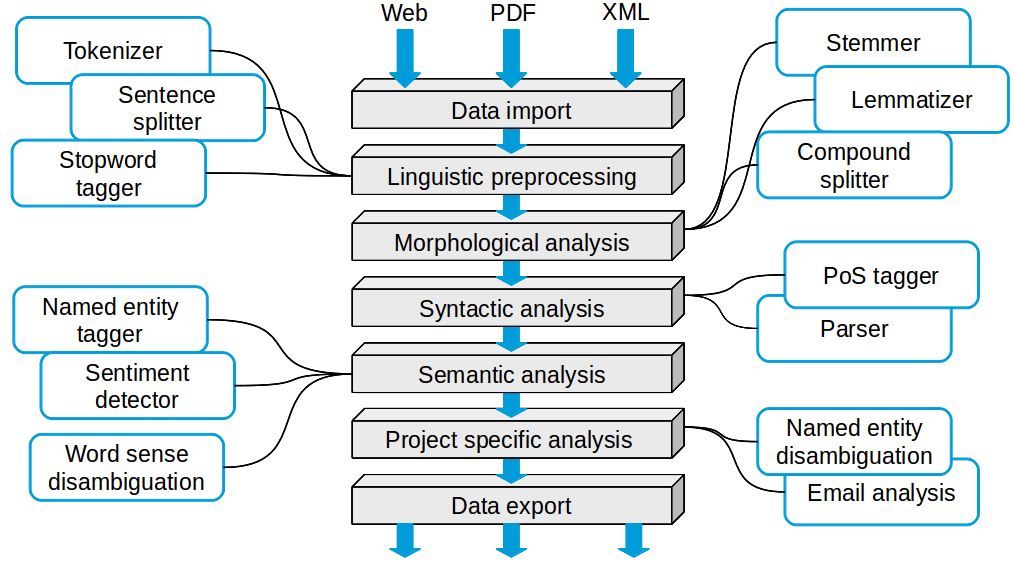
\includegraphics[width=1\textwidth]{fig/dkpro-pipeline.png}
    \caption[Short caption]{DKPro Core Pipeline}
    \label{fig:dkpro-pipeline}
\end{figure}


